\chapter{State-of-the-Art}\label{chap:state-art}

Surveillance measures (currently taken);
development of vaccines to protect humans is one central pillar of why the constant; ensure adequate hygiene, know and be alert to symptoms; vaccinate animals if possible and necessary --> control/surveillance of zoonoses is crucial \\

SARS-CoV-2 high similarity to SARS-CoV virus \\ animal origin is suspected (!)
	globally, in science, advances in bioinformatics: new surveillance techniques, e.g. clinical testing for self-monitoring \\
	systematic global collection of data that allows health professionals and policymakers to react with appropriate measures at hand to protect the public


molecular surveillance studies: genetic analysis is an integral part of animal disease surveillance.

surveillance systems include classical phylogenetic methods to genotype novel emerging strains, classify viral lineages or assess tree topologies to distinguish between novel and emerging strains

approaches to assess correlations between similarities of nucleotide sequences and related epidemiological characterstics

investigate spatio-temporal and evolutionary dynamics of the virus isolates in a disjointed analytical framework


\section{High-throughput Technologies in Diagnostic Virology}

\subsection{Overview of NGS Platforms and Applications}
% table of Illumina, ONT ...

\begin{figure}
	\centering
	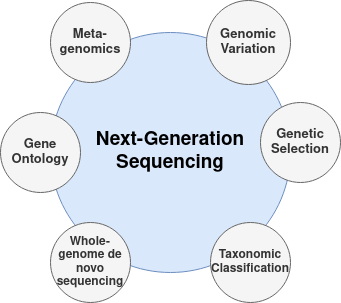
\includegraphics[width=0.5\textwidth]{media/other/ngs.png}
	\caption{Overview of Applications of Next-Generation Sequencing Technologies in diagnostic virology.}
	\label{fig:ngs}
\end{figure}

\subsection{Detection of Viral Pathogens}
- NGS-based methods: VIDISCA protocol for SARS-CoV in 2004
- metagenomics-based strategies: higher sensitivity (compared to microarray-based assays), detect full spectrum of viruses
- NGS-based: Illumina GA platform for detection of new viruses (influenza A) and de novo assembly (only works with high enough number of reads generated)
- bats: coronavirus consensus PCR and unbiased HTS (high-throughput pyrosequencing) -> reveal presence of sequences of new coronavirus related to SARS-CoV

\subsection{Data Analysis Issues}

no standardization of techniques \\
no knowledge sharing/best practices/common source of knowledge \\
livestock diseases do not receive much attention from bioinformaticians and therefore not enough monitoring;
although in regions where outbreaks have larger impacts on economy and other fields, the surveillance is crucial for prevention and control.

This emphasizes the importance of free and easy-access platforms like Galaxy that entitle professionals to analyse their samples. Technical know-how to develop and 
maintain servers for analysis of NGS data is not a global standard and also not needed everywhere when multidisciplinary approaches can be shared through platforms.

costs are relatively high, especially for countries or health organizations in development countries that are still affected by diseases they want to monitor

format of sequencing data -> data accuracy
%%%%%%%%%%%

Illumina shows low coverage of AT rich regions~\cite{harismendy2009evaluation}

* chimerical sequences (artifacts originating from joining sequences), point mutations, insertions/deletions which occur during reverse transcription, PCR amplification or sequencing itself
* cleaning step or filtering phase removes low-quality reads from the dataset, while the error correction separates true variants from those due to experimental noise. -> idea that errors are randomly distributed with low frequency, and real mutations are clustered and their abundance are quantified

Each application of software with NGS data requires expertise in resolving limitations and drawbacks of specific methods. This in turn requires bioinformatic skills and the careful interpretation of results. Still, NGS provides a large pool of methods which eases the tasks, although available algorithms for genome assembly and amplicon analysis have drawbacks and limitations~\cite{finotello2012comparative}.


% \subsubsection{OIE/FAO: OFFLU}
% WOAH/FAO: Network of Expertise on Animal Influenza
% WHO: GISRS (Global Influenza Surveillance and Response System) for human influenza,
% WHO: FluNet
% WHO: GISAID (Global Initiative on Sharing All Influenza Data)
% \cite{daniels2023health}

\section{NGS Methods for Poxviruses}

difference/similarities between monkeypox, goat pox, sheep pox etc. \\
advances in surveillance (4 genera of poxviruses are zoonotic and may infect humans)

classification based on phenotypic characteristics.

\subsection{Poxviruses}
2 subfamilies, one infects vertebrates and one infects insects
-> 10 genera infect vertebrates

characteristic ITR that is left out in other pipelines (Yale University primer scheme starts after and ends before ITR)

with monkeypox outbreak in 2022, professionals of the field had the event to examine another pox virus, seeing similarities among pox viruses motivates to extend existing pipelines for data analyses to work with samples of all pox viruses

one poxvirus to mention in more detail:
% \subsection{Lumpy Skin Disease Virus}\label{sec:LSDV}
Lumpy Skin Disease (LSD) is caused by the virus belonging to the Capripoxvirus (CaPV) genus within the family Poxviridae, subfamily Chordopoxvirinae~\cite{walker2019changes}. The LSDV genome is a double-stranded linear DNA molecule of circa 151 kilobasepairs in length. It contains between 147 and 156 open reading frames. With a sequence identity of over 96\% with the other CaPV genus members sheep pox and goatpox, the lSDV genome is very similar to the other CaPV genomes~\cite{tulman2001genome}. These three viruses of the capripoxvirus genus are the most serious poxvirus diseases of livestock in terms of economic losses in the case of an outbreak. 

One strain of LSDV that has been extensively studied is the Neethling strain, first isolated in Kenya in 1958. It constitutes the strain used for the live-attenuated vaccine that is widely used for cattle against LSDV outbreaks. Similar to other poxviruses, the LSDV genome consists of a central coding region which is bounded by two identical inverted terminal repeat (ITR) regions with a length of circa 2,400 basepairs at both ends of the genome. This is a key characteristic to consider during reconstruction of the genome. 

capripox not transmissable to humans -> NOT a zoonosis

viral disease that affects cattle, transmission through blood-feeding insects such as ticks or some species of mosquitoes and flies. \\
* symptoms \\
vaccination programme (mass-vaccination by EU commission protecting >1.8million cattle)\\
spreading in African countries, since 2012 present in middle east to south-east europe

Zoonotic: A disease of humans caused by pathogen coming from non-human host and vice versa.

Transmission modes, limited host range 


\subsection{Application of NGS Technologies in Poxvirus Diagnostics}

https://www.sciencedirect.com/science/article/pii/S0166093422000118 explains Primer scheme and why tiling amplicon approach makes sense even for large genome size of CaPV genome and complex structure with repetitive ITR regions


\section{NGS Methods for Avian Influenza Virus}\label{sec:AIV}
\subsection{Avian Influenza Virus}

informally known as bird flu, the avian influenza is a viral infectious disease whose hosts are wild waterbirds. \\
occurring in two variants determining the severeness, therefor low/highly pathogenic and in a variety of subtypes, that are composed by two viral segments H1-H16 in combination with N1-N11 \\

* symptoms

* LPAIV, HPAIV

* Etiology: virus composition, taxonomy, origin, mutation rates

Human Influenza Virus:
AIV has more subtypes as there are more prevalent subtypes in many different populations; more variants

\subsection{Application of NGS Technologies in Avian Influenza Virus Diagnostics}

%%%%%
SARS-CoV-2 tracking is of huge global interest, resulting in a highly regarded topic with ongoing scientific activity in terms of publications \\
includes established institutions in bioinformatics that hand out approaches, guidelines, recommendations to govern outbreaks of viral livestock diseases. includes comprehensive pipelines for bioinformaticians, veterinarians and other health professionals.
major platforms that offer exhaustive approaches to analyse genomic samples from infected stock. \\

efforts for end-to-end tools and pipelines for sequencing data

INSaFLU, ViReflow? (SARS-CoV-2 samples) \\
 VAPOR (ref datasets) \\

* INSaFLU (inside the flu) -> for influenza, NGS towards metagenomic virus detection, routine genomic surveillance, 

* Nextstrain -> for RT SARS-CoV-2, Influenza, Ebola pathogen populations 
* Kraken2 -> taxonomic sequence classifier (using database and k-mers of FASTA sequences)
* VirFind (by Arkansas High Performance Computing Center) -> for fasta/Illumina fastq files, to detect new samples (trimming, mapping to ref, de novo assembly, Blastn, Blastx)
* ARTIC Network -> RAMPART for Ebola, yellow fever virus (read assignment, mapping, phylogenetic analysis on ONT data)
* IRIDA -> Integrated Rapid Infectious Disease Analysis for NGS data e.g. de novo assembly (FLAsh, SPAdes, Prokka)


tracking viruses using genomic sequence data collection; effective surveillance does not require exhaustive case surveillance, instead the collection of enough data from representative populations. This enables health professionals to detect newly evolved variants and to monitor trends in the circulating variants.\\
wastewater